\section{Results} \label{sec:results}

We are now in a position to examine the limitations of action-based modelling posed in the introduction (see Section \ref{sec:intro}) using our \RM{} machinery. We explore: (i) unbiased estimates, (ii) the role of the survey volume, (iii) imperfect selection functions, (iv) measurement uncertainties and what happens if the actual (v) DF or (vi) Potential are not spanned by the space of models. We do not explore the breakdown of the assumption that the system is axisymmetric and
in steady state. With the exception of the test suite on measurement uncertainties in Section \ref{sec:results_errors}, we assume that phase-space uncertainties are negligible. All tests are also summarized in Table \ref{tbl:tests}. 

%====================================================================

%FIGURE: width of likelihood propto 1/sqrt(N)

\begin{figure}[!htbp]
\plotone{figs/sqrtNiso_Stddev_Vs_N.eps}
\caption{The width of the \pdf{} (see Equation \ref{eq:prob}) for two fit parameters found from analyses of 132 mock data sets vs. the number of stars in each data set. (The mock data was created according to the model parameters given in Test \ref{test:sqrtNiso} in Table \ref{tbl:tests}.) The relative standard error (SE) was found from a Gaussian fit to the marginalized \pdf{} for each model parameter. As can be seen, for large data samples the width of the \pdf{} scales with $1/\sqrt{N_{*}}$ as expected.} 
\label{fig:sqrtNiso}
\end{figure}

%====================================================================

%====================================================================

%FIGURE: central limit theorem is satisfied

\begin{figure}[!htbp]
\centering
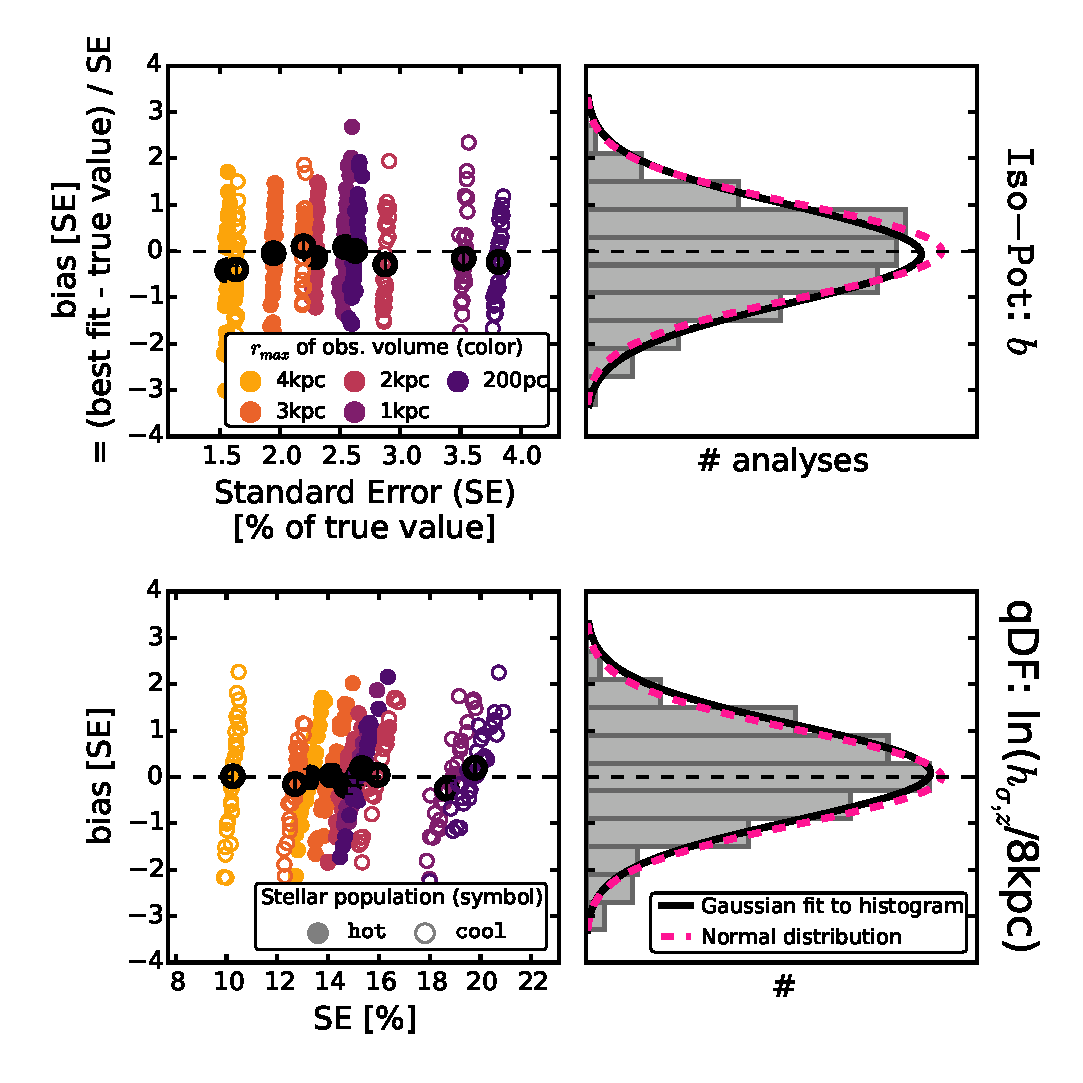
\includegraphics[width=\columnwidth]{figs/isoSph_CLT_2.eps}
\caption{(Un-)bias of the parameter estimates. Maximum likelihood estimators converge to the true true parameter values with Gaussian errors for large numbers of data points. To test that these conditions are satisfied for \RM{}, we create 320 mock data sets, which come from two different stellar populations and five spherical observation volumes (see legends). (All model parameters are summarized in Table \ref{tbl:tests} as Test \ref{test:isoSph_CLT}.) Bias and relative standard error (SE) are derived from the marginalized \pdf{} for two model parameters (isochrone scale length $b$ in the first row and qDF parameter $h_{\sigma,z}$ in the second row). The second column displays a histogram of the 320 offsets. As it closely follows a Normal distribution, our modelling method is therefore well-behaved and unbiased. The black dots show the mean offset and SE for the 32 analyses belonging to one model.}
\label{fig:isoSph_CLT}
\end{figure}

%====================================================================

%====================================================================

%FIGURE: Does shape and position of obs. volume matter?


\begin{figure*}[!htbp]
\centering
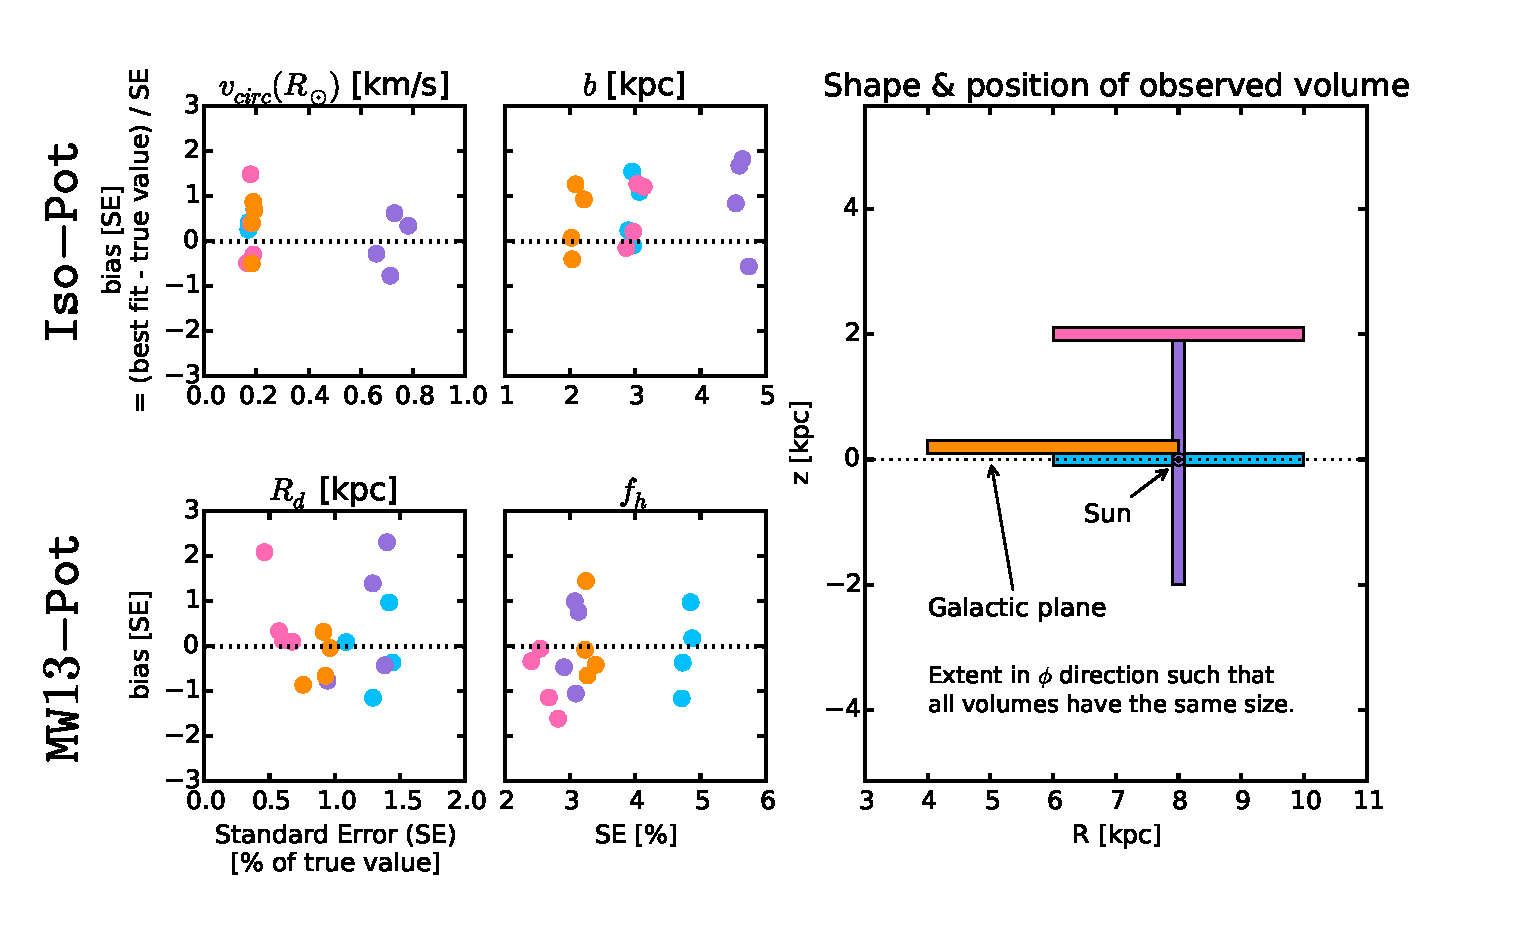
\includegraphics[width=0.7\textwidth]{figs/wedFlexVol_bias_vs_SE.eps}
\caption{Bias vs. standard error in recovering the potential parameters for mock data stars drawn from four different wedge-shaped test observation volumes within the Galaxy (illustrated in the right panel; the corresponding analyses are colour-coded) and two different potentials (\texttt{Iso-Pot} and \texttt{MW13-Pot} from Table \ref{tbl:referencepotentials}; see also Test \ref{test:wedFlexVol} in Table \ref{tbl:tests} for all model parameters used). Standard error and offset were determined from a Gaussian fit to the marginalized \pdf{}. The angular extent of each wedge-shaped observation volume was adapted such that all have the volume of $4.5~\text{kpc}^3$, even though their extent in $(R,z)$ is different. Overall there is no clear trend, that an observation volume around the Sun, above the disk or at smaller Galactocentric radii should give remarkably better constraints on the potential than the other volumes.}
\label{fig:wedFlexVol_bias_vs_SE}
\end{figure*}


%====================================================================

